\section*{5.4 传统对当方阵}
具有相同主项和相同谓项的标准式直言命题,可能在量上有所不同, 189 或者在质上有所不同,也可能在质与量上都不同。先前的逻辑学家称之为对当关系(opposition),各种对当关系之间有很重要的真值联系。

\section*{A.矛盾关系(Contradictories)}
两个命题之间具有矛盾关系,如果一个是另一个的拒斥(denial)或否定(negation),也就是说,它们既不能同真也不能同假。显而易见,如果两个标准的直言命题的主项相同、谓项也相同,而质、量都不同,那么,它们就是矛盾的。例如 A 和 O 就是这样的,比如:

所有法官都是律师。

与

有法官不是律师。

这两个命题的质与量都是对立的,显然它们是矛盾的。其中之一为真时,另一个恰恰为假。

同理, E 和 I 也是这样:

没有政客是理想主义者。

与

这两个命题的质与量都是对立的,因而它们是矛盾的。用公式表示就是: "所有 $S$ 是 $P$"的矛盾命题是"有 $S$ 不是 $P$",而"没有 $S$ 是 $P$"的矛盾命题是"有 S 是 P "; A 和 O 互为矛盾, E 和 I 互为矛盾。

\section*{B.反对关系(Contraries)}
两个命题之间具有反对关系,如果它们不能同时为真,也就是说,可以由一个的真推出另一个的假。例如,"得克萨斯队将在比赛中战胜俄克拉何马队"与"俄克拉何马队将在比赛中战胜得克萨斯队"就是反对的;如果两个命题中的一个(当然指的是在同一场比赛中)是真的,那么另一个必定为假。但它们不是矛盾的,因为如果他们打成平手,两个命题就同时为假。具有反对关系的两个命题,不能同时为真,但可以同时为假。传统逻辑或曰亚里士多德逻辑认为,如果两个直言命题都是全称的,其主、谓项分别相同而质不同,那么它们就是互相反对的。 ${ }^{[1]} \mathrm{A}$ 命题和相应的 E命题不能同时为真,却可以同时为假,所以它们之间是反对关系,例如 "所有诗人都是懒汉"与"没有诗人是濑汉"。

如果 A 命题或者 E 命题是必然真的一一即在逻辑上或数学上为真一一那么,说它们是互相反对的就是不正确的。例如,"所有三角形都是四边形"与"没有三角形是四边形"。如果一个命题是必然真的一一不可能为假的一一那么,它就没有反对命题,因为互相反对的命题可以同假。我们把既非必然真也非必然假的命题称为偶真的(contingent)。如果一个 A 命题和一个 E 命题都是偶真的,并且它们有相同的主项和相同的谓项,那么,说它们是反对的就是正确的。本章其他部分的讨论都假定 A和 E 是偶真的。

\section*{C.下反对关系(Subcontraries)}
两个命题之间具有下反对关系,如果它们不能同假,但可以同真。传统上认为,如果两个直言命题都是特称的,其主、谓项分别相同而质不同,那么它们之间是下反对关系。也就是肯定了 I 和 O 命题,可以同真但不可同假,如:

有钻石是珍贵的石头。

有钻石不是珍贵的石头。\\
必定是下反对的。\\
如果 I 和 O 必然为假,那么,说它们是下反对的就不正确。例如"有正方形是圆"与"有正方形不是圆"。如果一个命题必然为假——也就是说,不可能为真一一那么它就不会有下反对的对立面。因为,两个互为下反对的命题是可以同真的。当然,如果 I 和 O 都是偶真的,就可以同真。与反对关系一样,本章其他部分的讨论亦假定 I 和 O 都是偶真的。

\section*{D.差等关系(Subalternation)}
如果两个命题有相同的主项和相同的谓项,并且它们的质相同(即都是肯定的或者都是否定的),但量不同(即一个为全称,另一个为特称),那么,它们之间的关系就是差等关系。例如,A 命题:

\section*{所有蜘蛛都是八脚动物。}
有一个相应的 I 命题:

有蜘蛛是八脚动物。

191 而 E 命题:

\begin{displayquote}
没有鲸是鱼。
\end{displayquote}

也有一个相应的 O 命题:

\section*{有鲸不是鱼。}
此前用于说明命题间对当关系的例子都有"对立"(disagreement)的含义。但这里使用的"对当关系"是个专业术语,也适用于并不存在"对立"含义的情况。在上面的例子中,A 命题和相应的 I 命题之间不"对立",E命题和 O 命题之间也不"对立",但它们却都具有一种特殊的"对

当关系"。全称命题与相应的特称命题之间的对当关系叫做差等关系。在一对相应的命题中,比如刚才给出的两对,全称命题叫做"上位式",特称命题叫做"下位式"。

传统上认为,在差等关系中,上位的真蕴涵下位的真。举例来说,从全称肯定命题"所有鸟是有羽毛的"可以得出特称肯定命题"有鸟是有羽毛的";而从全称否定命题"没有鲸是鱼"可以得出特称否定命题"有鲸不是鱼"。但下位并不蕴涵上位。从特称肯定命题"有动物是猫"不能得出全称肯定命题"所有动物是猫"。同样,从特称否定命题"有动物不是猫"当然也不能推出"没有动物是猫"的结论。

\section*{E.对当方阵}
命题之间这四种对当关系——矛盾关系、反对关系、下反对关系以及上位与下位之间的差等关系——可以用一个重要且广为应用的图示来表示,称为"对当方阵",见图 5-1。\\
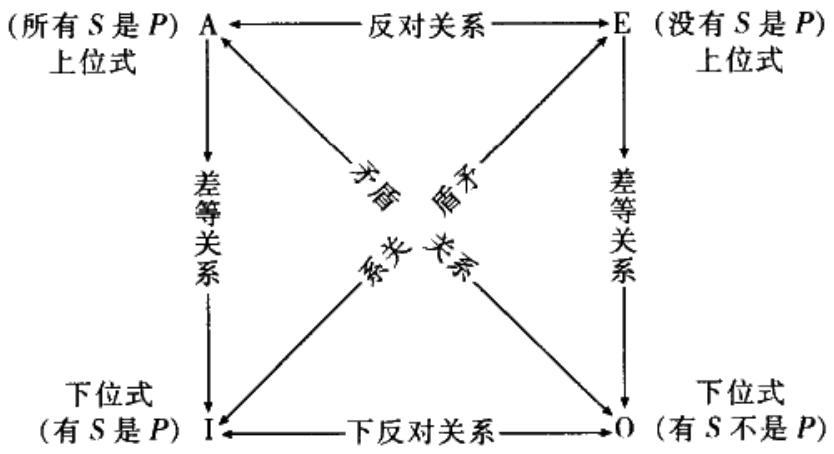
\includegraphics[max width=\textwidth, center]{2025_05_15_6a28331d5e7c993ad07ag-238}

图 5-1\\
展示在对当方阵中的关系,为把握论证的一些基本形式的有效性提供了一个逻辑基础。如果我们按照惯例将论证分为直接推论和间接推论,那就更容易理解了。

任何论证都是从一个或多个前提得出一个结论。包括一个以上前提的推论叫做间接推论,例如三段论,其结论就是从第一个前提经由第二个前提为中介得出的。而如果从唯一的前提出发,不经过任何中介推得结论,这样的推论叫做直接推论。容易见得,许多非常有用的直接推论,可从传统对当方阵所包含的知识中获得。

下面看一些例子。如果以 A 命题为前提,根据对当方阵,可以有效

地推出相应的(即主、谓项分别相同的)O命题为假。从同样的前提也可以有效地推出相应的 I 命题为真。当然,从 I 命题的真不能推出相应的 A命题为真,但可以推出其矛盾命题 E 为假。以对当方阵为基础,还可以得到许多这样的直接推论。给定任一标准式直言命题的真假情况,就可以直接得到其他某个或者所有其他相应命题的真假情况。基于对当方阵的直接推论可以列表如下:

如果 A 真,那么, E 假、 I 真、 O 假;\\
如果 E 真,那么, A 假、 I 假、O 真;\\
如果 I 真,那么,E 假,A、O 真假不定;\\
如果( )真,那么,A 假,E、I 真假不定;\\
如果 A 假,那么,O 真,E、I 真假不定;\\
如果 F 假,那么, I 真, A 、O 真假不定;\\
如果 I 假,那么, A 假、 E 真、O 真;\\
如果 O 假,那么, A 真、 E 假、 I 真。 ${ }^{[2]}$
\footnotetext{(1)5.6 节将对此传统观点作批判性讨论。}
\footnotetext{(2)纽约州立大学 Brockport 分校的约瑟夫•吉尔伯特(Joseph Gilbert)教授在其私人通信中提到,一个命题真假不定时,可能会产生一些意想不到的结论。如果已知 A 命题真假不定,我们可以推出其矛盾命题 O 必定也是真假不定的,因为如果知道 O命题为真或为假,那么 A 命题的真假也就能够确定了。对于 E命题及其矛盾命题也是这样。一般说来,如果一个命题是真假不定的,那么,它的矛盾命题必然也真假不定。如果 A 命题真假不定,其反对命题 E 必定为假,因为如果 E 为真,那么 A 就不是真假不定的。同理,如果已知 A 命题真假不定,那么相应的 I 命题必定为真。} 